\documentclass[12pt, a4paper, one side]{article}
\usepackage[utf8]{inputenc}
\usepackage[french]{babel}
\usepackage{listings}
\usepackage{color}
\usepackage{graphicx}

\title{Documentation de validation}
\author{}
\date{}


\definecolor{dkgreen}{rgb}{0,0.6,0}
\definecolor{gray}{rgb}{0.5,0.5,0.5}
\definecolor{mauve}{rgb}{0.58,0,0.82}

\lstset{frame=tb,
    language=java,
    aboveskip=3mm,
    belowskip=3mm,
    showstringspaces=false,
    columns=flexible,
    basicstyle={\small\ttfamily},
    numbers=none,
    numberstyle=\tiny\color{gray},
    keywordstyle=\color{blue},
    commentstyle=\color{dkgreen},
    stringstyle=\color{mauve},
    breaklines=true,
    breakatwhitespace=true,
    tabsize=3
}

\begin{document}

\maketitle

\begin{center}
    Valentin Laclautre, Anthony Dard, Damien Trouche, Martin Gangand, Basel Darwish Jzaerly
\end{center}

\tableofcontents

\newpage

\section{Introduction}

Cette documentation a pour but de présenter tout les différents tests créés pendant le projet.
Pour chaque test, on décrira son fonctionnement, et on expliquera son intérêt. On présentera aussi
la manière de l'exécuter, ainsi que son importance dans la couverture de test.

\section{Bon fonctionnement de decac}

\subsection{Détection des différentes options données}

Ce premier test a pour but de vérifier que le parsage des différentes options données en ligne
de commande lors de l'execution de decac est correct. Pour cela on fait appel à la classe \textit{CompilerOptions}
et on regarde la valeur des differents attributs donnant si une option est présente ou non. On vérifie aussi que si l'on
donne des options incorrects, une erreur est levée.

\section{Fichiers *.deca pour tester la syntaxe contextuelle du langage Deca}
Nous trouvons dans test/deca/context/ des fichiers qui respectent la syntaxe du langage Deca et d'autres qui ne la respectent pas.
Pour chaque programme valide (qui se trouve dans valid/custom), nous avons en commentaires une déscription du programme,
le résultat attendu, et ensuite le programme.
La structure est la même pour les fichiers invalides (qui se trouvent dans invalid/custom). Nous voyons en commentaires pourquoi le programme ne compile pas.

\begin{lstlisting}
// affect-compatible-type-value.deca
// Description: Affectation d'une valeur sur un type different mais compatible.
// Resultats:
//    Ligne 12: affichage 1.
//    Cela est permis selon la page 75 du poly.
{
   // Doit être accepté.
    float a = 1;
    print(a);
}
\end{lstlisting}

\begin{lstlisting}
// affect-incompatible-type-value.deca
// Description:
//    Affectation et typage sur valeur
// Resultats:
//    Ligne 12: Affectation d'une valeur sur un type incompatible.
//    Cela est permis selon la page 75 du poly.
// Remarque : la réciproque est acceptée.
{
   // Doit être refusé.
    int a = 1.2;
}
\end{lstlisting}

\section{Tests syntaxiques}
\subsection{Lancer les tests pour le Lexer}
Nous avons créé plusieurs tests unitaires deca pour notre lexer. Pour les lancer de manière automatique, il faut se placer dans le répertoire \newline
\textit{gl28/src/test/java/fr/ensimag/deca/syntax} et exécuter \textbf{TestLex.java}. Ce programme utilisant JUnit nous permet de vérifier que les tokens obtenus sont effectivement ceux que nous attendions. Pour cela nous vérifions les tokens un par un, et lorsque qu'un token diffère du token attendu, une erreur est levée.

Cette méthode de test étant très manuelle puisqu'il faut vérifier les tokens un par un, nous nous sommes limités à 5 tests qui concernent des tests basiques par manque de temps. Par exemple, nous utilisons un programme vide, un autre qui affiche "hello world", ou encore un test sur une chaîne de caractère incomplète.

\subsection{Lancer les tests pour le Parser}
Il est également possible de tester notre parser avec une large batterie de tests. Le script \textbf{basic-synt.sh} du répertoire \textit{gl28/src/test/script} permet de lancer ces tests. Plus précisément, pour chaque test, le programme \textbf{ManualTestSynt.java} est appelé et il permet d'utiliser le parser sur le fichier passé en argument. Contrairement aux tests du Lexer où nous vérifions le résultat du test, ici nous regardons seulement si le programme renvoie une erreur ou pas, ce sont des tests Oracle. Ainsi, pour les résultats des tests dans le répertoire invalid, nous attendons une erreur du parser.

Notre batterie de tests portant sur la syntaxe se trouve dans le répertoire \textit{gl28/src/test/deca/syntax}. Ensuite vous retrouvez un dossier pour les tests invalides, c'est à dire qui ne respectent pas la syntaxe de la grammaire, et un dossier pour les test valides. Dans ces dossiers nous avons ajouté un répertoire \textit{custom} pour y ajouter tous nos tests personnalisés comme vous pouvez le voir ci dessous.

\subsection{Arborescence des tests syntaxiques}
Le répertoire \textit{syntax} se trouve dans le dossier \textit{gl28/src/test/deca}.
\begin{center} 
    \includegraphics[scale=0.7]{treesyntax.png} 
\end{center}

\subsubsection{Répertoire \textit{valid/custom}}
Ce répertoire contient plusieurs dossiers qui correspondent chacun à une catégorie de test différente. Quatre de ces dossiers concernent les fonctions d'affichage (print, printx, println, printlnx). Nous avons tenté de tester toutes les possibilités de la grammaire. On y retrouve par exemple des affichages d'entiers, de flottants, ou encore le résultats d'opérations arithmétiques.

\subsubsection{Répertoire \textit{valid/custom/return}}
Ce répertoire contient des fichier deca qui utilise un return. On peut par exemple retourner le résultat d'opérations arithmétiques unaires ou binaires, tout comme des chaînes de caractères.

\subsubsection{Répertoire \textit{valid/custom/while}}
Ce répertoire contient le même genre de test que ceux pour le return. C'est à dire que nous utilisons une grande variété de conditions différentes.

\subsubsection{Répertoire \textit{valid/custom/if\_then\_else}}
Ce répertoire de tests porte sur différentes utilisations de la condition if. Par exemple, la condition peut porter sur le résultat d'une opération booléenne, ou sur celui d'une comparaison entre deux entiers. Nous vérifions aussi la bonne implémentation du bloc else if.

\subsubsection{Répertoire \textit{valid/custom/object}}
Ce répertoire assez conséquent permet de tester le parser avec l'utilisation d'objets et l'appel de méthodes. Par exemple, nous créons des classes qui héritent d'une autre classe. Nous vérifions aussi que des mots clés comme "instanceof", "this", ou "new" ne génèrent pas d'erreurs.

\subsubsection{Répertoire \textit{invalid}}
L'arborescence des tests qui sont syntaxiquement invalides est légèrement différente. La majorité des tests se trouvent dans le répertoire \textit{syntax/invalid/custom}. On y fait par exemple des tests dans lesquels il manque une parenthèse, une opérande, ou encore des fichiers contenant une CircularInclude.

Il y a tout de même deux répertoires pour les tests sur les objets et sur l'option -java. Ces derniers tests sont les mêmes que ceux du répertoire valid, à ceci près qu'ils sont incorrects.


\section{Tests contextuels}
Nous avons ensuite créé une autre batterie de tests qui porte sur l'étape B, et notamment sur la vérification des trois passes.

\subsection{Lancer les tests contextuels}
Nous avons un script pour lancer tous nos tests, il se trouve dans le répertoire gl28/src/test/script. Pour le lancer il suffit d'écrire ./basic-context.sh dans le terminal, de la même façon que le script de la partie précédente. Ce programme va lancer le fichier ManualTestContext et vérifie les trois passes pour tous nos fichiers de tests Oracle. Ces tests sont organisés selon l'aspect de la grammaire traité comme le décrit l'arborescence ci-dessous.

\subsection{Arborescence des tests contextuels}
Le répertoire \textit{context} se trouve dans le dossier \textit{gl28/src/test/deca}.
\begin{center}
    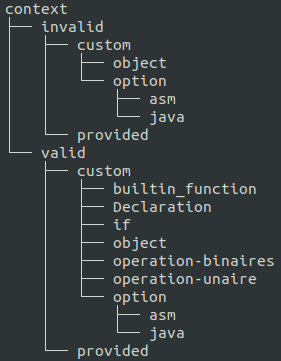
\includegraphics[scale=0.7]{treecontext.png}
\end{center}

\subsubsection{Répertoire \textit{valid}}
Dans ce répertoire on retrouve nos tests personnalisés dans le dossier \textit{custom}. Ici aussi, nous avons créé plusieurs répertoires qui concernent les différents aspects vérifiés.

\begin{flushleft}
Le répertoire builtin\_function vérifie le bon fonctionnement des fonctions d'affichage (print, printx, println, printlnx).
\end{flushleft}
\begin{flushleft}
Le répertoire \textit{Declaration} permet de regrouper nos tests avec différents types de déclarations de variables. Nous testons par exemple le bon fonctionnement de ConvFloat en additionnant un entier et un flottant. Dans ce cas, la conversion de l'entier en flottant est implicite.
\end{flushleft}
\begin{flushleft}
Le répertoire \textit{if} utilise plusieurs conditions différentes, par exemple on peut faire des opérations sur des booléens, tout comme des comparaisons entre des flottants.
\end{flushleft}
\begin{flushleft}
Le répertoire \textit{operation-unaire} utilise les opérateurs "-" et "not". Il est important de vérifier cela car par exemple "not" ne s'applique que sur des booléens, alors que "-" ne s'applique que sur des entiers et des flottants.
\end{flushleft}
\begin{flushleft}
Le répertoire \textit{operation-binaires} utilise les différentes opérations arithmétiques comme l'addition, la multiplication, la division, la soustraction, ou le modulo. Nous vérifions aussi le bon fonctionnement de la conversion implicite d'un entier en flottant.
\end{flushleft}
\begin{flushleft}
Enfin, le répertoire \textit{option} regroupe les tests sur l'option -java que nous avons implémentée. Seul le dossier \textit{asm} est lancé pour le script basic-context.sh.
\end{flushleft}

\subsubsection{Répertoire \textit{invalid}}
De la même manière que pour les tests de la partie syntaxique, la plupart des tests invalides se trouvent directement le répertoire \textit{context/invalid/custom}. Nous avons ajouté un dossier pour l'option et un autre pour ce qui concerne la partie objet.

\section{Tests de génération de code}
Dans la continuité des tests précédents, nous avons créé des tests valides et invalides pour la génération de code pour la machine ima. Ces tests sont dans le répertoire \textit{gl28/src/test/deca/codegen}, puis on distingue les tests valides et invalides.

\begin{flushleft}
Nous avons choisi de créer des tests de type "boîte noire", ainsi pour chaque fichier deca, nous avons créé un fichier .res contenant le résultat attendu dans le même répertoire. Le script vérifie alors que le résultat obtenu par l'exécution du fichier généré par le compilateur decac est le même que le résultat qui est attendu.
\end{flushleft}

\subsection{Lancer les tests de génération de code}
Le script qui permet de lancer l'exécution de tous les tests est \textbf{basic-gencode.sh} qui se trouve dans le répertoire \textit{gl28/src/test/script}.

\subsection{Arborescence des tests de génération de code}
Le répertoire \textit{codegen} se trouve dans le dossier \textit{gl28/src/test/deca}.
\begin{center}
    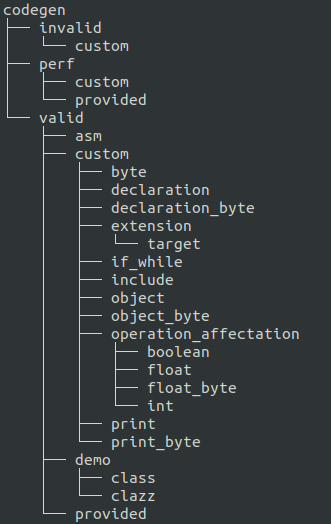
\includegraphics[scale=0.6]{treecodegen.png}
\end{center}
\subsubsection{Répertoire valid/custom}
Nos tests personnalisés se trouvent dans le répertoire \newline
\textit{gl28/src/test/deca/codegen/valid/custom}. On y retrouve plusieurs catégories de tests comme pour les parties précédentes.

\begin{flushleft}
Le répertoire déclaration contient toute sorte de déclarations. Par exemple, ont peut simplement déclarer des entiers ou des flottants, mais aussi déclarer une variable qui est le résultat d'une opération.
\end{flushleft}

\begin{flushleft}
Le répertoire extension permet vérifier le bon fonctionnement de l'insertion de code java dans deca. Par exemple, il est possible d'importer une librairie java et de l'utiliser pour retourner un résultat. L'explication des tests concernant notre extension BYTE se trouve dans la documentation de l'extension.
\end{flushleft}

\begin{flushleft}
Le répertoire \textit{if\_while} utilise simplement des blocs if et while. Ces tests très simples nous permettent de nous assurer que la génération de code est bonne.
\end{flushleft}

\begin{flushleft}
Le répertoire \textit{include} permet de tester l'utilisation du mot clé include. Par exemple, nous vérifions qu'il est possible de créer une classe dans un fichier decah, puis de l'importer dans un fichier deca tout en pouvant l'utiliser.
\end{flushleft}

\begin{flushleft}
Le répertoire \textit{object} regroupe tous les tests de la partie avec objet. Nous manipulons des classes, tout en utilisant le principe d'héritage. Nous utilisons aussi des upcasts et des downcasts. Nous testons également que dans une classe fille il est possible de redéfinir un champs de même nom que dans la classe mère.
\end{flushleft}

\begin{flushleft}
Le répertoire \textit{operation\_affectation} contient les répertoires \textit{boolean}, \textit{int}, et \textit{floats}. Nous utilisons des affectations un peu particulières. Par exemple, on vérifie l'affection du résultat d'une opération de comparaison à un booléen, ou encore l'affection à un entier du résultat d'une opération avec plusieurs opérande et dont le résultat est un flottant, dans ce cas la conversion en float est implicite.
\end{flushleft}

\begin{flushleft}
Enfin, le répertoire \textit{print} affiche sur la sortie standard différentes opérandes. Ces dernières peuvent être le résultat d'une opération arithmétique, une chaîne de caractère, ou même la concaténation des deux.
\end{flushleft}

\subsubsection{Répertoire invalid/custom}
Nos tests personnalisés se trouvent dans le répertoire \newline
\textit{gl28/src/test/deca/codegen/invalid/custom}. Nous y testons par exemple des casts avec des objets incompatibles, ou encore l'appel d'une fonction qui doit retourner une valeur mais ne retourne rien.

\section{Objectifs de ces tests}
Notre objectif était de réaliser des tests pour nous assurer que tout fonctionne correctement. Ainsi, nous avons construit des tests en nous servant de la grammaire. Nous comptons pas moins de 500 tests pour la vérification syntaxique et contextuelle, ce qui nous permet d'avoir une base solide concernant les étapes A et B.

\begin{flushleft}
Concernant l'étape C, nous avons opté pour des tests "boîte noire" car nous pensons que c'est un bon moyen de valider le bon fonctionnement de notre compilateur. La vérification de cette étape est primordiale car c'est le résultat final qui en sort.
\end{flushleft}
\begin{flushleft}
Nous pouvons dire que d'une manière générale, ces tests nous ont été très utiles. En effet, il est important de tester nos fonctionnalités au fur et à mesure de leur implémentions pour savoir ce qui ne fonctionne pas, ce qui fonctionne correctement, et ce qui pourrait être amélioré. De plus, cela nous a permis de résoudre un grand nombre de bugs qui n'auraient sans doute pas été détectés sans une large couverture de tests.
\end{flushleft}
\begin{flushleft}
Pour chacun des tests nous affichons un message pour savoir si le test a été validé ou non. De plus les scripts de l'étape A et B utilisent des compteurs, de cette manière nous avons le nombre de tests validés pour chaque répertoire, ainsi que le nombre total de tests validés par rapport au nombre total de test exécutés.
\end{flushleft}

\section{Limites de la base de tests}
Durant ce projet nous avons essayé de tester le plus grand nombre d'aspects possible de la grammaire. Cependant, notre résultat de couverture Jacoco est de 77\%, ce qui signifie que certaines parties ne sont pas vérifiées. Il est alors possible de rajouter des tests concernant les étapes A, B, ou C. Pour cela, il suffit d'ajouter des fichiers deca dans les dossiers existants des répertoires \textbf{syntax}, \textbf{context}, et \textbf{codegen}. Puis, il suffit de lancer les scripts correspondant pour obtenir les résultats.

\section{Gestion des risques et gestion des rendus}
\subsection{Risque d'isolement pour cause de covid}
Il était évident qu'en cette période, le risque qu'au moins une personne de notre groupe soit positive au covid était élevé. Conscients de ce risque dès le début, nous avons décidé que dans ce cas nous adopterions un mode de travail mixte, c'est à dire à la fois en présentiel et en distanciel via discord pour les personnes malades.

\begin{flushleft}
Cette situation s'est produite puisque une semaine après avoir commencé le projet Basel s'est retrouvé isolé à cause du covid. Cette situation n'était pas idéal pour lui car il a travaillé pendant 2 semaines seul chez lui.
\end{flushleft}

\subsection{Risque de propager des bugs}
Lors d'un projet comme celui-ci, il est possible de propager des bugs sur le git du projet. Pour essayer de réduire au maximum ce risque, nous avons mis en place plusieurs actions.

\begin{flushleft}
Tout d'abord, nous avons créé plusieurs branches de travail. Chaque branche correspondait à un aspect du projet, c'est à dire la partie sans objet, avec objet, ou encore l'extension. Cela nous a permis d'éviter de devoir faire beaucoup de merge intermédiaires, et donc de réduire la possibilité de faire des erreurs.
\end{flushleft}
\begin{flushleft}
De plus, avant d'apporter des modifications au dépôt git, nous nous assurions que le projet se compilait bien avec la commande mvn compile.
\end{flushleft}

\subsection{Risque de ne pas rendre un produit à temps}
\begin{flushleft}
Le risque d'oublier une date de rendue est basique mais il est bien présent. Pour éviter cela, le logiciel de planification développé par Anthony nous a permis de nous imposer des dates de fin maximum.
\end{flushleft}
\subsection{Risque de ne pas respecter la syntaxe DECA et les contraintes conextuelles}
\begin{flushleft}
Un aspect critique sur la partie technique du projet concerne le respect de la syntaxe DECA. Pour limiter ce risque, nous avons décidé d'attacher une grande importance aux tests. C'est pourquoi nous avons implémenté un ensemble représentatif de programmes de tests, c'est à dire faisant intervenir tous les tokens et toutes les règles de la grammaire concrète.
\end{flushleft}
\begin{flushleft}
Dans cette même logique, nous avons créé une large batterie de tests pour vérifier le respect des contraintes contextuelles. Nous avons tenté de faire intervenir le plus de règles de la grammaire et erreurs contextuelles possibles.
\end{flushleft}
\end{document}
